\ofsubsection{Races}
%
\ofquote{"I suppose you think we look ...odd, don’t you? That’s fine. We Guado are used to that sort of thing.
	But if you ask me, you humans look absolutely disgusting. Still, what does it matter? Such nonsense is beneath us, no?
	Once, a human child simply looked at me and then burst into tears. That hurt."}{Female Guado}\\
%
\vfill
%
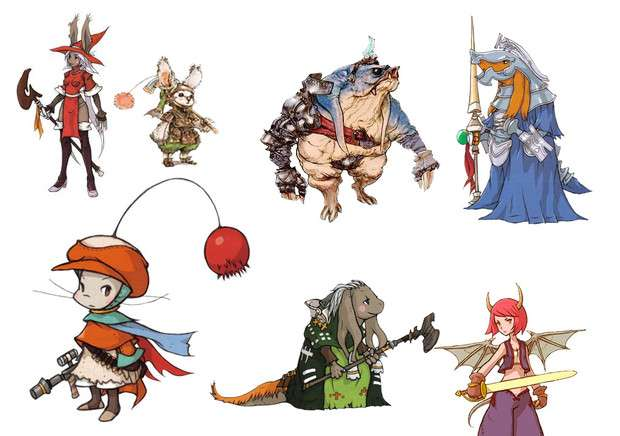
\includegraphics[width=\columnwidth]{./art/races/races.jpg}
%
\vfill
%
We generally differentiate between two kinds of living beings: characters, which by default we assume to be human and monsters, which we assume to be similar to animals.
As in the real world, one can identify different tribes and races within those groups and for monsters we present a wide variety of different species in the bestiary.
In the following, we will explore character races that are fictional, but resemble humans in both appearance and intelligence.
These, so-called \accf{Humanoid Races} can be interesting for both players and game masters, because they increase the diversity of the game world, while still fulfilling the same roles as humans. 
%
\vfill
%
\ofquote{"We dwarves have a saying: Be bold. But if things look grim, run away and be bold another day instead."\\}{Male Dwarf}\\\\
%
As the GM, you can create multiple humanoid races to make up the population of your world.
Usually, those races fall somewhere in-between humans and monsters.
On the one hand, they are intelligent, can interact and communicate with humans and create their own civilizations and technologies.
On the other hand, humanoid races can have a vastly different appearance, language, outlook and way of life compared to humans.  
Furthermore, races with a different anatomy might prefer living conditions that are unpleasant to humans, such as underwater, underground or on treetops.
Naturally, the existence of such different races will have consequences on the state of the world:
just as human tribes, different races may create conflicts and alliances within themselves and between each other.
Accordingly, each race will write its unique history and shape the world in its own regard.
%
\newpage
%
\ofquote{"I have to find out who I am. I'm scared. What if I'm not even human?"}{Vivi}\ofpar
%
As inhabitants of the game world, player characters can also be part of any humanoid race that exists in it.
Therefore, it is important that the GM briefly introduces the existing races to the players before they create their characters.  
When a player chooses his or her character to be from a non-human race, this usually implies the following consequences:  
firstly, it is important that the players consider their character's race and origin as part of their background story.
Furthermore, the appearance of a character will be heavily influenced by their race and they might show specific personality traits that are common within their people. 
During the adventure, party members of different races may be perceived and treated differently, depending on who they interact with.
%
\vfill
%
The choice of race should not fundamentally change the mechanics of the game for player characters.
Nevertheless, it is beneficial to explore gameplay elements that help players to consider their character's race when roleplaying.
Each race usually has at least one craft or discipline which they excel in, usually enabled by their unique anatomy or knowledge.
Such expertise can be expressed through race exclusive Talents, so-called \accf{Racial Talents}.
They work exactly as regular Talents, but are only available to characters of specific races.
When players create their characters, they can choose one Racial Talent for their character's race in addition to their regular Talent.
In the following, some example of humanoid races are given, which are inspired by races that appear in various Final Fantasy games.
They are to be understood as examples and GMs are not expected to include them as part of the world they create.
Their primary purpose is to provide inspiration to GMs that want to create their own races.
Finally, note that two Racial Talents are given for each example to allow players regardless of the chosen race.
%
\vfill
%
\ofboxwithtitle{Example: Racial Talents} 
{
	Kimahri Ronso is a guardian of Summoner Yuna, who he has sworn to protect her on her pilgrimage. 
	When a young boy named Tidus also tries to become her guardian, Kimahri decides to test his combat prowess.
	He hides on top of some ruins and waits for Tidus to walk by to surprise him.
	The GM asks both of them to make a check to decide whether the ambush is successful.
 	Kimahri has the Mighty Hunter racial talent for Ronso, so he gains Advantage on this check.
	He rolls [1,~5,~4] while Tidus only rolls [3,~2].
	The GM therefore decides that Tidus is taken off guard and Kimahri starts the ensuing battle with a surprise round.
}
%
\clearpage
%
%
\ofquote{"It takess a lot of nerve to call a Bangaa a lizard!"\\}{Male Bangaa}
%
\begin{center} 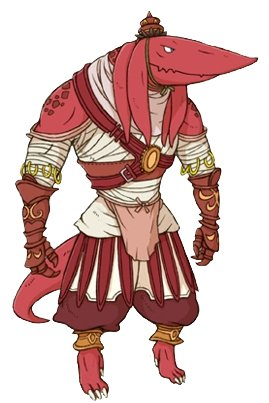
\includegraphics[width=0.88\columnwidth]{./art/races/bangaa.jpg} \end{center}
%
With their skin covered in scales, as well as their long heads and tails, \accf{Bangaa} clearly resemble reptiles.
Another notable trait are their four long ears which hang off from the sides of their faces.
Their impressive physique and unusual features make Bangaa appear intimidating towards other races.
Even though they are quite intelligent, the anatomy of their mouth makes it difficult for them to speak human languages properly.
Bangaa have no rigid societal structures.
They often travel or reside in big cities and have no problems with living among other races. 
Although Bangaa are traditionally a race of warriors, many have advanced beyond that and towards disciplines such as trade, politics or craftsmanship.
Most Bangaa shy away from Magic, but they make up for it with their physical strength and intelligence.
They also have a preference towards using well-crafted weapons and armor.
%
\\\\
%
\accf{Racial Talent - Regenerate:} Bangaa scales not only protect against incoming damage, but also help them to recover from injuries much more quickly.
After every successfully completed battle, you immediately regain an amount of HP equal to your current Level if you are not suffering KO. 
%
\\\\
%
\accf{Racial Talent - Brute Force:} As one of the most physically formidable races, you receive Advantage on checks related to lifting, moving, and other unopposed feats of strength.
%
%
\newpage
%
%
\ofquote{"Although we Guado differ from humans in appearance, our respect for the dead is the same."\\}{Male Guado}
%
\begin{center} 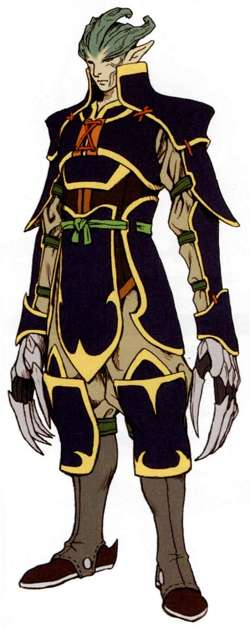
\includegraphics[width=0.5\columnwidth]{./art/races/guado.jpg} \end{center}
%
The most prominent features of \accf{Guado} are their long arms that end in claw-like fingers and their long ears.
Their hair grows out of their head in an unusual manner and is often compared to branches of a tree.
Guado are slightly thinner and more flexible than humans, which enables them to be surprisingly agile.
Nevertheless, they prefer wearing long clothes or heavy armor.
Guado usually build their settlements in natural environments such as forests or caverns.
They are a religious race that practices elaborate rituals to commemorate their dead.
The so-called Maester is the official religious and the de facto political leader of the tribe.
Guado are extremely well versed in Magic and prefer it to using advanced technology.
They believe themselves to be superior to other races and are in return perceived as arrogant by others.
%
\\\\
%
\accf{Racial Talent - Farplane:} Guado have a unique connection to the world of the dead, which they call the Farplane.
You can perform a 10 minute long ritual and if you successfully pass a check, you can speak to the ghost of a dead character.
The DC is determined by the GM, but it becomes easier the closer you are to the persons place of death and 
the closer your relationship with the dead person was.
%
\\\\
%
\accf{Racial Talent - Fleet of Foot:} Guadao receive Advantage on races and other opposed checks based on pure speed.
%
\clearpage
%
\ofquote{"A stuffed animal!? I'll have you know I'm a moogle, kupo!"}{Montblanc}
%
\begin{center} 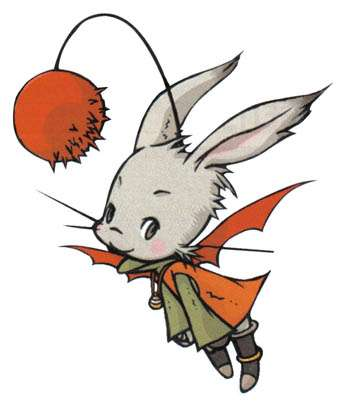
\includegraphics[width=0.8\columnwidth]{./art/races/moogle.jpg}  \end{center}
%
\accf{Moogle} are very short, usually no taller than 1u and have rather high pitched voices.
With their long ears and their fur, which can be of almost any color, they resemble rabbits.
In addition they have small wings on their back as well as an antenna on their head, with a large ball of fur at its end.
This "pom pom" is very sensitive to touch and thus Moogle are usually very protective of it.
Moogle are very diverse: while some live in hidden forest tribes, others prefer traveling alone or living in large cities.
They are an ambitious race that loves to explore and discover different disciplines. 
While they have traditionally relied on Magic to survive, modern Moogles have also become skilled tinkerers, artists, traders and even warriors.
Their diet mostly consists of nuts and plants, as they rarely touch meat at all.
Moogle are generally perceived as kind and trustworthy, but are often not taken seriously due to their appearance.
%
\\\\
%
\accf{Racial Talent - Glide:} Using their wings, Moogle can fly up to 0.5u above the ground and can cover a distance of up to 10u before landing.
While flying, they can move only half as fast compared to their walking speed.
Furthermore, Moogle can glide down from heights of up to 10u without taking any damage.
%
\\\\
%
\accf{Racial Talent - Mognet:} Due to your magical abilities, you are able to telepathically communicate with any known Moogle or any willing non-Moogles you share a close bond with, for example someone in your party.
%
\newpage
%
\ofquote{"It's hard when everyone thinks of you as a genius"\\}{Ezel}\\
%
\begin{center} 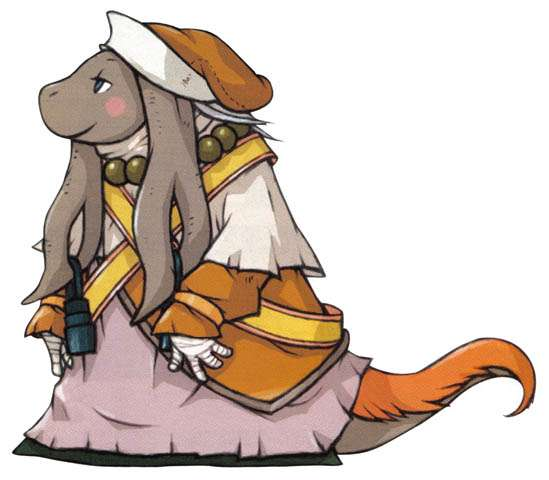
\includegraphics[width=\columnwidth]{./art/races/numou.jpg} \end{center}
%
\accf{Nu Mou} are slightly shorter than most other races and the color of their smooth skins can vary greatly between its members.
They have rather round bodies and faces that together with their long tails, remind of canine animals.
Their long ears branch off towards the end, leaving large holes that they often decorate with earrings.
The average Nu Mou life span is also significantly longer than any other race, with some living for more than 300 years.
It is believed that Nu Mou are by far the oldest race in existence, that once ruled over the most rich and powerful civilizations.
Nowadays, the members of their race are scattered across the world with barely any cohesion.
They have always been highly skilled Magic users, but more and more Nu Mou also show interest in the research of alchemy, astronomy and monster taming.
Most of them also tend to be introverted and focused on one area of expertise, which is why other races perceive the Nu Mou as odd, but harmless beings.   
%
\\\\
%
\accf{Racial Talent - Ancient Wisdom:}  Bits and pieces of ancient Nu Mou wisdom have survived through the centuries and are still known among its members.
Accordingly, you are capable of reading and understanding almost any old language or dialect regardless of how long it has not been in use.
%
\\\\
%
\accf{Racial Talent - Nu Mou Noble:} As a member of a noble clan of Nu Mou, you are more knowledgable in the way of the magical Arts. You can always identify any spell or magical affect similar to one of your own and receive Advantage when attempting to identify unfamiliar magics.
%
\clearpage
%
\ofquote{"You have angered Kimahri! The spirits of the Ronso will guide Kimahri’s spear!"}{Kimahri}
%
\begin{center} 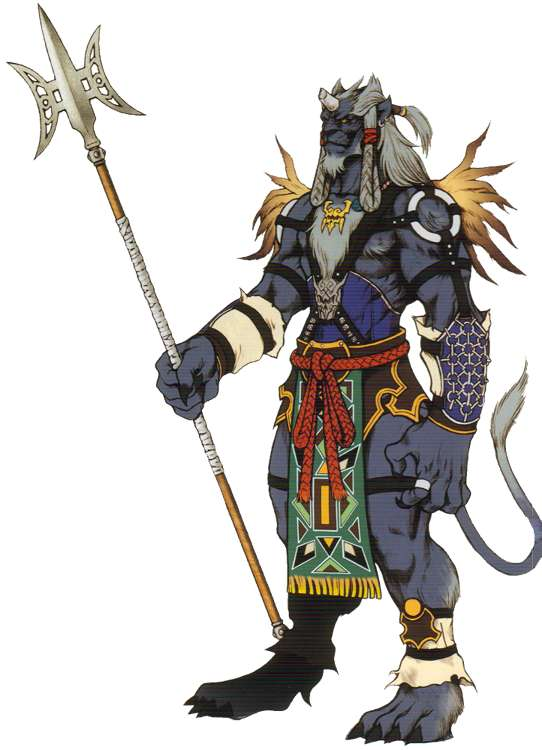
\includegraphics[width=\columnwidth]{./art/races/ronso.jpg} \end{center}
%
\accf{Ronso} appear like a mixture between humans and lions. 
While they show many feline features such as claws and a tail, their mannerisms are closer to humans.
However, Ronso differ from both with their blue-colored fur and their horn on their forehead.
They prefer light clothing, as their fur already covers their entire body.
Ronso tribes prefer to live in cold climates, usually on top of mountains, which they consider to be sacred.
They are a race of warriors first and foremost who rarely deal with Magic or technology.
Ronso tend to be religious and take special pride in their horns, which they understand to be the source of their strength.
Still, they are generally indifferent to outsiders and occasionally engage with other races and civilizations on friendly terms.
Therefore, Ronso are perceived as a kind, but primitive people by other races. 
%
\\\\
%
\accf{Racial Talent - Tough Hide:} Their thick fur allows Ronso to be comfortable regardless of their surroundings.
You are not slowed down by difficult terrain such as swamps or snow and you do not require shelter even under extreme weather conditions.
%
\\\\
%
\accf{Racial Talent - Mighty Hunter:} As a carnivorous species, the Ronso have become hunters par-excellence. You gain advantage on rolls involving both stalking prey and avoiding notice.
%
\newpage
%
\ofquote{"The Viera may begin as part of the Wood, but it is not the only end that we may choose."}{Fran}
%
\begin{center} 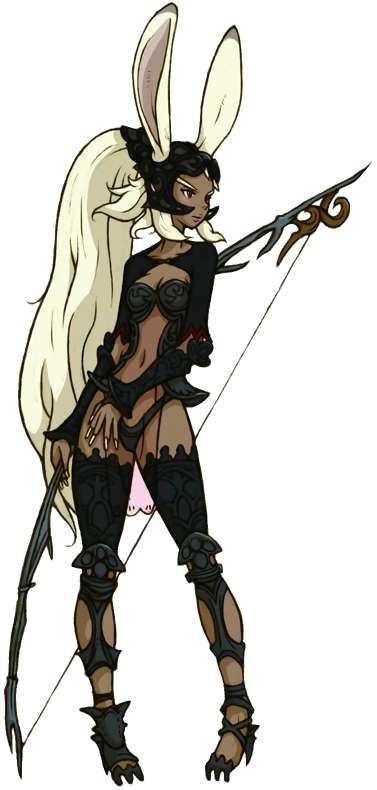
\includegraphics[width=0.58\columnwidth]{./art/races/viera.jpg} \end{center}
%
\accf{Viera} look similar to humans, except for a few distinguishing features: 
their long ears are covered with fur and their claw-like hands and pointed feet are reminiscent of feline limbs.
Most Viera wear gloves and heeled shoes that are made to fit their unique anatomy.
In general, they prefer light and revealing clothing that does not impede their movement.
Viera tribes live in forests that are closed off to the rest of the world.
They not only consider the forest to be their own, but they also feel a spiritual connection to the flora and fauna.
As such, they usually do not engage with other races and are hostile towards outsiders.
Viera who decide to leave the forest are immediately considered as exiles and treated like outsiders.
While Viera tribes mostly consist of hunters and gatherers, some also have a strong affinity towards Magic.
Exiled Viera are often not as proficient in their traditional disciplines, but may posses a wider set of skills due to their experiences in other civilizations.
%
\\\\
%
\accf{Racial Talent - Naturally Perceptive:} Viera have much sharper senses compared to other races.
You gain Advantage on all checks that involve noticing nearby sounds, smells, traces and movements.
%
\\\\
%
\accf{Racial Talent - Outcast of The Wood:} As one of the Viera who has left their ancestral home, you have learned to survive by honing your wildcraft. You are adept at identifying healing herbs, setting up camp, and disguising your past whereabouts and gain Advantage on such checks.
%
\clearpage
%
\ofquote{"When a person has someone they care about that much, giving their life is sometimes the least they can do. And maybe that's what makes us human."}{Vincent}
%
\begin{center} 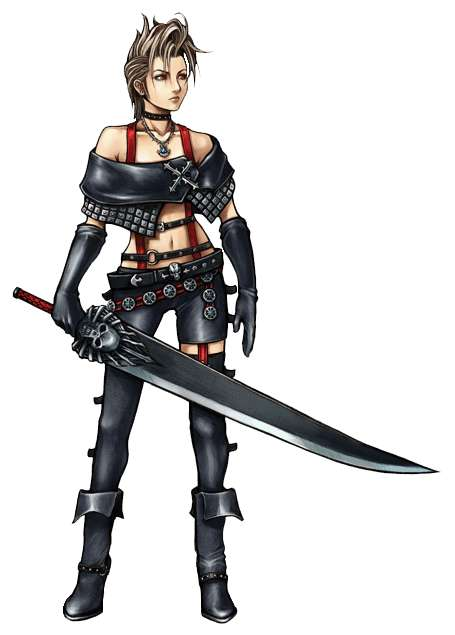
\includegraphics[width=0.9\columnwidth]{./art/races/human.jpg} \end{center}
%
\accf{Humans}, by any other name, are just as adaptive and adventurous as their real-world counterparts. 
Hailing from seemingly every world in the multiverse, these beings have a tendency to be ambitious, cunning, inquisitive, and have made for as many heroes as they have villains! 
Indeed, their drive for self improvement and to simply know is seemingly boundless. 
As a testament to their drive and power, humanity is one of the most prevalent species to be found on many planets and planes.
One of the humanities strengths is the staggering variety of languages and social institutions they exhibit. 
This is said to account for their conviction in individual freedom, though it also results in a relative lack of solidarity and group cohesion.
\\\\
\accf{Racial Talent - Will to Power:} Some people are driven by the desire for perfection and self-improvement, letting nothing stand in their way save their own moral compasses. You are one such person, with the blood of conquerors coursing through your veins. In situations requiring leadership or negotiation.
\\\\
\accf{Racial Talent - By the Skin of My Teeth:} Be it a blessing of the Fates, or merely a reflection of their inner essence, many humans have an uncanny knack at surviving the greatest perils and in this you are no exception. Whenever you pass a check that you had Disadvantage on, you gain Advantage on the next check you make.
%
\pagebreak\\
%
\ofquote{"yawn ...You want to fight? After this map, maybe..."\\}{Male Miqo'te}
%
\begin{center} 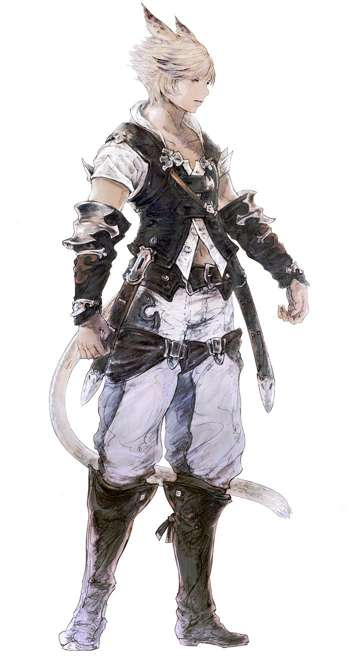
\includegraphics[width=0.7\columnwidth]{./art/races/miqote.jpg} \end{center}
%
A species of humanoid felines, the \accf{Miqo'te} are much fewer in number and more insular than other races. 
With their pronounced ears and fur-covered tails, Miqo'te appear as a mixture between humans and cats.
However, unlike other races, they prefer a clothing style that is very similar to human fashion.
Most Miqo'te live in isolated tribes with strict hierarchical structures, but some of them have also have also successfully integrated themselves into other cultures.
Traditionally, the Miqo'te worship the Sun and the Moon as their gods.
A wide range of personalities is represented within the race: some are quick-witted, prone to action, and bore easily while others are more reserved and brooding, yet tenacious. 
Miqo'te are well suited to various environments, be it jungle, desert, or plains and have remarkable skills in hunting in fishing due to their high dexterity.
\\\\
\accf{Racial Talent - Catlike Reflexes:} Your greatest blessings are your eyes, your ears, and your tail. 
You receive Advantage on rolls that involve stalking prey and balancing, while ignoring Disadvantage due to darkness.
\\\\
\accf{Racial Talent - Nine Lives:} Sometimes you just can't keep a good Mithra down. 
Whenever you suffer KO, you can recover from it by resting for 1 hour instead of requiring a full night's sleep.
%
%
\clearpage
